\documentclass[11pt,a4paper]{article}

\usepackage{array}
\usepackage{graphicx}
\usepackage{tabularx}

\usepackage[margin=1.0in]{geometry}

\begin{document}
\title{BatSignal:\\System Design Document}
\author{
	Bryan Young\\youngb2@wit.edu \and
	Joe Moraal\\moraalj@wit.edu\\ \and
	Zach Thornton\\thorntonz@wit.edu \and
	Computer Science 2015 \\
	Wentworth Institute of Technology
}
\date{\today}

\maketitle
\newpage

\tableofcontents{}
\newpage


\section{Introduction}

\subsection{Purpose and Scope}
\textnormal{This document describes the hardware and software components of the BatSignal distributed sensor network. This document is intended for use by developers implementing BatSignal.}

\subsection{Project Executive Summary}
% This section provides a description of the project from a management perspective and an overview of the framework within which the conceptual system design was prepared.  If appropriate, include the information discussed in the subsequent sections in the summary.
\textnormal{The BatSignal network is designed to function as a rapid response alert system capable of identifying, by sensor ID, situations of distress or emergency. The system passively collects audio captures from the sensors and analyzes them for keywords or phrases. When the system detects a matching keyword or phrase it dispatches an email to a list of administrators and displays a notification on the system console. \\
The system is designed to be physically scaled according to the needs of the location of installation. Controller nodes are installed at or near administrative areas with sensor nodes installed in patient rooms, inhabited spaces, common areas, etc. Communication propagate through the BatSignal mesh network allowing nodes to communicate with the controller despite physical distance.}

\subsubsection{System Overview}
% This section describes the system in narrative form using non-technical terms.  It should provide a high-level system architecture diagram showing a subsystem breakout of the system, if applicable.  The high-level system architecture or subsystem diagrams should, if applicable, show interfaces to external systems.  Supply a high-level context diagram for the system and subsystems, if applicable.  Refer to the requirements trace ability matrix (RTM) in the Functional Requirements Document (FRD), to identify the allocation of the functional requirements into this design document.
\begin{center}
	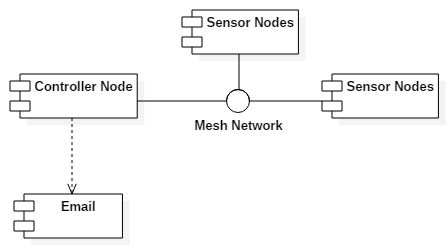
\includegraphics[scale=0.75, keepaspectratio=true]{Graphics/SimpleOverview.png}
\end{center}

\subsubsection{Design Constraints}
% This section describes any constraints in the system design (reference any trade-off analyses conducted such, as resource use versus productivity, or conflicts with other systems) and includes any assumptions made by the project team in developing the system design.

\subsubsection{Future Contingencies}
%This section describes any contingencies that might arise in the design of the system that may change the development direction.  Possibilities include lack of interface agreements with outside agencies or unstable architectures at the time this document is produced.  Address any possible workarounds or alternative plans.

\subsection{Points of Contact}
% This section provides the organization code and title of the key points of contact (and alternates if appropriate) for the information system development effort.  These points of contact should include the Project Manager, System Proponent, User Organization, Quality Assurance (QA) Manager, Security Manager, and Configuration Manager, as appropriate.


\subsection{Project References}
% This section provides a bibliography of key project references and deliverables that have been produced before this point.  

\subsection{Glossary}
% Supply a glossary of all terms and abbreviations used in this document.  If the glossary is several pages in length, it may be included as an appendix.

\subsubsection{System Specific Definitions}
\begin{center}
\begin{tabularx}{\textwidth}{ | l | X | }
	\hline
	\multicolumn{2}{ | c | }{\textbf{System Specific Definitions}} \\
	\hline
		& \\
	\hline
\end{tabularx}
\end{center}

\subsubsection{Technical Definitions}
\begin{center}
\begin{tabularx}{\textwidth}{ | l | X | }
	\hline
	\multicolumn{2}{ | c | }{\textbf{Technical Definitions}} \\
	\hline
	CPU		& Central Processing Unit \\
	GPIO	& General Purpose Input Output \\
	GPU		& Graphical Processing Unit \\
	MHz		& Mega-Hertz \\
	USB		& Universal Serial Bus \\
	SoC		& System on a Chip \\
	\hline
\end{tabularx}
\end{center}

\subsubsection{Industry Definitions}
\begin{center}
\begin{tabularx}{\textwidth}{ | l | X | }
	\hline
	\multicolumn{2}{ | c | }{\textbf{Industry Definitions}} \\
	\hline
	B.A.T.M.A.N		& Better Approach to Mobile Ad-hoc Networking \\
	\hline
\end{tabularx}
\end{center}

\subsection{Document Organization}
% This section describes the organization of the Systems Design Document.
\textnormal{In the following sections this document will define the overall system architecture followed by more detailed hardware and software architectures. }

\section{System Architecture}
% In this section, describe the system and/or subsystem(s) architecture for the project.  References to external entities should be minimal, as they will be described in detail in Section 6, External Interfaces.
\begin{center}
	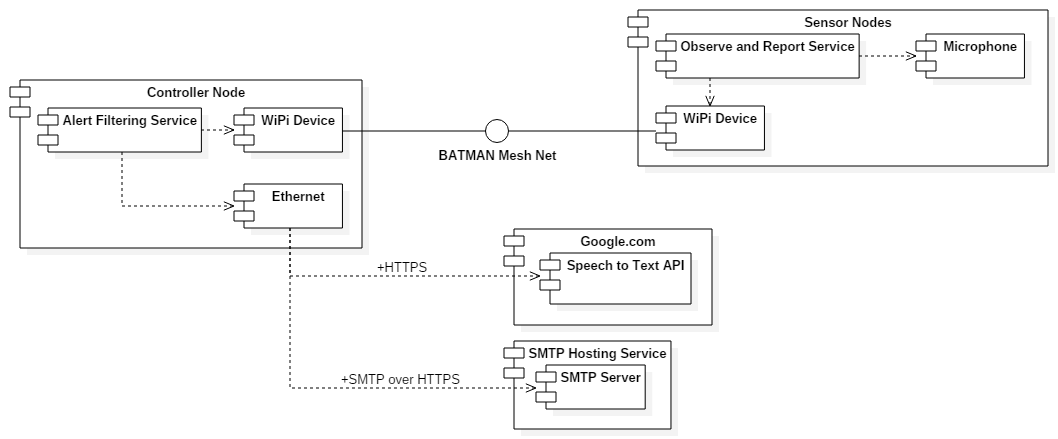
\includegraphics[width=\textwidth, keepaspectratio=true]{Graphics/SystemArchitecture.png}
\end{center}

\subsection{System Hardware Architecture}
% In this section, describe the overall system hardware and organization.  Include a list of hardware components (with a brief description of each item) and diagrams showing the connectivity between the components.  If appropriate, use subsections to address each subsystem.

\subsection{System Software Architecture}
% In this section, describe the overall system software and organization.  Include a list of software modules (this could include functions, subroutines, or classes), computer languages, and programming computer-aided software engineering tools (with a brief description of the function of each item).  Use structured organization diagrams/object-oriented diagrams that show the various segmentation levels down to the lowest level.  All features on the diagrams should have reference numbers and names.  Include a narrative that expands on and enhances the understanding of the functional breakdown.  If appropriate, use subsections to address each module.
% Note: The diagrams should map to the FRD data flow diagrams, providing the physical process and data flow related to the FRD logical process and data flow.


\subsection{Internal Communications Architecture}
% In this section, describe the overall communications within the system; for example, LANs, buses, etc.  Include the communications architecture(s) being implemented, such as X.25, Token Ring, etc.  Provide a diagram depicting the communications path(s) between the system and subsystem modules.  If appropriate, use subsections to address each architecture being employed.
% Note: The diagrams should map to the FRD context diagrams.

\section{Human-Machine Interface}
% This section provides the detailed design of the system and subsystem inputs and outputs relative to the user/operator.  Any additional information may be added to this section and may be organized according to whatever structure best presents the operator input and output designs.  Depending on the particular nature of the project, it may be appropriate to repeat these sections at both the subsystem and design module levels.  Additional information may be added to the subsections if the suggested lists are inadequate to describe the project inputs and outputs.
\textnormal{The BatSignal Distributed sensor network expects }

\subsection{Inputs}
%This section is a description of the input media used by the operator for providing information to the system; show a mapping to the high-level data flows described in Section 1 .2.1, System Overview.  For example, data entry screens, optical character readers, bar scanners, etc.  If appropriate, the input record types, file structures, and database structures provided in Section 3, File and Database Design, may be referenced.  Include data element definitions, or refer to the data dictionary.
%Provide the layout of all input data screens or graphical user interfaces (GUTs) (for example, windows).  Provide a graphic representation of each interface.  Define all data elements associated with each screen or GUI, or reference the data dictionary.
%This section should contain edit criteria for the data elements, including specific values, range of values, mandatory/optional, alphanumeric values, and length.  Also address data entry controls to prevent edit bypassing.
%Discuss the miscellaneous messages associated with operator inputs, including the following:
% •	Copies of form(s) if the input data are keyed or scanned for data entry from printed forms
% •	Description of any access restrictions or security considerations
% •	Each transaction name, code, and definition, if the system is a transaction-based processing system

\subsection{Outputs}
% This section describes of the system output design relative to the user/operator; show a mapping to the high-level data flows described in Section 1.2.1.  System outputs include reports, data display screens and GUIs, query results, etc.  The output files are described in Section 3 and may be referenced in this section.  The following should be provided, if appropriate:
% •	Identification of codes and names for reports and data display screens
% •	Description of report and screen contents (provide a graphic representation of each layout and define all data elements associated with the layout or reference the data dictionary)
% •	Description of the purpose of the output, including identification of the primary users
% •	Report distribution requirements, if any (include frequency for periodic reports)
% •	Description of any access restrictions or security considerations

\section{Detailed Design}
% This section provides the information needed for a system development team to actually build and integrate the hardware components, code and integrate the software modules, and interconnect the hardware and software segments into a functional product.  Additionally, this section addresses the detailed procedures for combining separate COTS packages into a single system.  Every detailed requirement should map back to the FRD, and the mapping should be presented in an update to the RTM and include the RTM as an appendix to this design document.

\subsection{Hardware Detailed Design}
% A hardware component is the lowest level of design granularity in the system.  Depending on the design requirements, there may be one or more components per system.  This section should provide enough detailed information about individual component requirements to correctly build and/or procure all the hardware for the system (or integrate COTS items).
% If there are many components or if the component documentation is extensive, place it in an appendix or reference a separate document.  Add additional diagrams and information, if necessary, to describe each component and its functions, adequately.  Industry-standard component specification practices should be followed.  For COTS procurements, if a specific vendor has been identified, include appropriate item names.  Include the following information in the detailed component designs (as applicable):
% •	Power input requirements for each component
% •	Signal impedances and logic states
% •	Connector specifications (serial/parallel, 11-pin, male/female, etc.)
% •	Memory and/or storage space requirements
% •	Processor requirements (speed and functionality)
% •	Graphical representation depicting the number of hardware items (for example, monitors, printers, servers, I/O devices), and the relative positioning of the components to each other
% •	Cable type(s) and length(s)
% •	User interfaces (buttons, toggle switches, etc.)
% •	Hard drive/floppy drive/CD-ROM requirements
% •	Monitor resolution

\subsubsection{Raspberry Pi 2}
\textnormal{Both versions of BatSignal nodes target the Raspberry Pi model 2 board. These systems have the following capabilities:
\begin{center}
\begin{tabularx}{\textwidth}{ | l | X | }
	\hline
	\multicolumn{2}{ | c | }{\textbf{Raspberry Pi 2 Specifications}} \\
	\hline
	Cost:				& \$35 USD \\
	\hline
	SoC:				& Broadcom BCM2836 \\ 
	\hline
	CPU:				& 900MHz quad-core ARM Cortex-A7 \\
	\hline
	GPU:				& Broadcom VideoCore IV, OpenGL ES 2.0, OpenVG 1080p30 H.264 high-profile encode/decode \\
	\hline
	Memory (SDRAM)iB:	& 1024 MiB \\
	\hline
	USB 2.0 Ports:		& 4 (via intergrated USB hub and LAN9512) \\
	\hline
	Onboard Storage:	& Micro Secure Digital / MicroSD slot \\
	\hline
	Onboard Network:	& 10/100 wired Ethernet RJ45 \\
	\hline
	Real-time Clock:	& None \\
	\hline
	Power Ratings:		& 650 mA, (3.0 W) \\
	\hline
	Power Source: 		& 5 V (DC) via Micro USB type B or GPIO header \\
	\hline
	Size:				& 85.0mm x 56.0 mm x 17mm \\
	\hline
	Weight:				& 40g \\
	\hline
\end{tabularx}
\end{center}
}

\subsubsection{Wi-Pi WLAN Module}
\textnormal{
\begin{center}
\begin{tabularx}{\textwidth}{ | l | X | }
	\hline
	\multicolumn{2}{ | c | }{\textbf{Wi-Pi WLAN Module Specifications}} \\
	\hline
	Cost: 				& \$15.52 \\
	\hline
	Physical Interface: & USB 2.0 \\
	\hline
	Wireless Standards: & IEEE 802.11n \\ 
						& Backward compatible with IEEE 802.11g and IEEE 802.11b \\
	\hline
	Transmission Speed: & 11b: 1/2/5.5/11 Mbps \\
						& 11g: 6/9/12/18/24/36/48/54 Mbps \\
						& 11n: up to 150 Mbps \\
	\hline
	Frequency Range: 	& 2.4 to 2.4835 GHz \\
	\hline
	Working Channel: 	& 1 to 13 \\
	\hline
	Transmit Power: 	& 20dBm (max) \\
	\hline
	Security Features: 	& WPA-PSK/WPA2-PSK \\
						& WPA/WPA2 \\
						& 64/128/152 bit WEP Encryption \\
	\hline
\end{tabularx}
\end{center}
}

\subsubsection{Microphone}
\textnormal{
\begin{center}
\begin{tabularx}{\textwidth}{ | l | X | }
	\hline
	\multicolumn{2}{ | c | }{\textbf{Microphone Specifications}} \\
	\hline
		& \\
	\hline
\end{tabularx}
\end{center}
}

\subsection{Software Detailed Design}
% A software module is the lowest level of design granularity in the system.  Depending on the software development approach, there may be one or more modules per system.  This section should provide enough detailed information about logic and data necessary to completely write source code for all modules in the system (and/or integrate COTS software programs).
% If there are many modules or if the module documentation is extensive, place it in an appendix or reference a separate document.  Add additional diagrams and information, if necessary, to describe each module, its functionality, and its hierarchy.  Industry-standard module specification practices should be followed.  Include the following information in the detailed module designs:
% •	A narrative description of each module, its function(s), the conditions under which it is used (called or scheduled for execution), its overall processing, logic, interfaces to other modules, interfaces to external systems, security requirements, etc.; explain any algorithms used by the module in detail
% •	For COTS packages, specify any call routines or bridging programs to integrate the package with the system and/or other COTS packages (for example, Dynamic Link Libraries)
% •	Data elements, record structures, and file structures associated with module input and output
% •	Graphical representation of the module processing, logic, flow of control, and algorithms, using an accepted diagramming approach (for example, structure charts, action diagrams, flowcharts, etc.)
% •	Data entry and data output graphics; define or reference associated data elements; if the project is large and complex or if the detailed module designs will be incorporated into a separate document, then it may be appropriate to repeat the screen information in this section
% •	Report layout

\appendix
\section{Appendix}

\end{document}